\documentclass[tikz]{standalone}

\usepackage{tikz}

\usetikzlibrary{arrows,automata, positioning}




\begin{document}



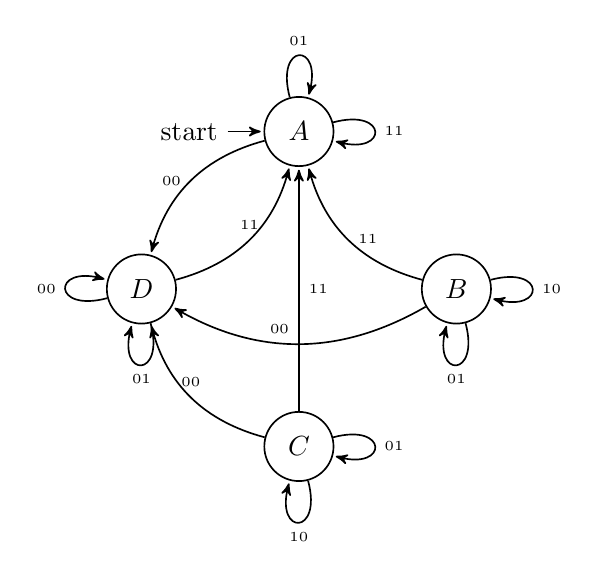
\begin{tikzpicture}[->,>=stealth',shorten >=1pt,auto,node distance=2.8cm,
                    semithick]



\node[state, initial] (1) at(0,2) {$A$};
\node[state] (2) at(2,0) {$B$};
\node[state] (3) at(0,-2) {$C$};
\node[state] (4) at(-2,0) {$D$};

\draw 
(1) edge[above, bend right, left=0.3] node{\tiny $00$} (4)
(1) edge[loop above] node{\tiny $01$} (1)
(1) edge[loop right] node{\tiny $11$} (1)

(2) edge[above left, bend left] node{\tiny $00$} (4)
(2) edge[loop below] node{\tiny $01$} (2)
(2) edge[loop right] node{\tiny $10$} (2)
(2) edge[right, bend left] node{\tiny $11$} (1)

(3) edge[above, bend left] node{\tiny $00$} (4)
(3) edge[loop right] node{\tiny $01$} (3)
(3) edge[loop below] node{\tiny $10$} (2)
(3) edge[right] node{\tiny $11$} (1)

(4) edge[loop left] node{\tiny $00$} (4)
(4) edge[loop below] node{\tiny $01$} (4)
(4) edge[above, bend right] node{\tiny $11$} (1)



;\end{tikzpicture}


\end{document}